\documentclass{article}

%
%	PAGE GEOMETRY
%
\usepackage{geometry}
\geometry{
	paperwidth=15cm, %7cm, %7cm, % 15cm
	paperheight=4cm,
	layouthoffset=0cm,
	layoutvoffset=0cm,
	hmargin={0cm,0cm},
	vmargin={0cm,0cm}
}
%

%
%	FILE ENCODING
%
\usepackage[utf8]{inputenc}
%

%
%	AMS STUFF
%
\usepackage{amsfonts}
\usepackage{amsthm}
\newtheorem{theorem}{Theorem}
%

%
%	ACRONYMS
%
\usepackage{acronym}
\acrodef{GA}{Genetic algorithms}
\acrodef{rmse}[error]{root-mean-square error}
\acrodef{GAPoly}[{\sc GAPoly}]{Genetic Algorithms for Polynomials}
%

%
%	FIGURE AND STUFF ENVIRONMENT
%
\usepackage{graphicx}
%

%
%	TIKZ AND RELATED STUFF
%
\usepackage{pgfplots}
\pgfplotsset{compat=newest}
\usepgfplotslibrary{statistics}
%
%
%%%%%%%%%%%%%%%%%%%%%%%%%%%%%%%%%%%%%%%%%%%%%%%%%%%%%%%%%%%%%%%%%%%%%%%%%
%
%	EMBEDDED DATASETS
%
\begin{filecontents}{inlambdas.dat}
2.474 2.460
2.414 2.392
2.414 2.392
2.414 2.392
2.407 2.392
2.407 2.392
2.317 2.331
2.351 2.331
2.330 2.331
2.314 2.318
2.251 2.318
2.251 2.318
2.251 2.318
2.275 2.318
2.275 2.318
2.275 2.318
2.275 2.318
2.275 2.296
2.275 2.296
2.268 2.296
2.268 2.296
2.268 2.296
2.225 2.296
2.225 2.296
2.225 2.296
2.225 2.296
2.225 2.296
2.225 2.296
2.225 2.268
2.225 2.268
2.225 2.268
2.225 2.261
2.225 2.261
2.225 2.261
2.225 2.261
2.225 2.261
2.225 2.261
2.225 2.261
2.225 2.261
2.225 2.261
2.225 2.261
2.225 2.261
2.225 2.261
2.225 2.261
2.225 2.261
2.225 2.261
2.225 2.261
2.225 2.261
2.225 2.261
2.225 2.261
2.225 2.261
2.225 2.261
2.225 2.261
2.225 2.261
2.225 2.261
2.225 2.261
2.225 2.261
2.225 2.261
2.225 2.261
2.225 2.247
2.225 2.247
2.200 2.247
2.200 2.247
2.200 2.247
2.200 2.247
2.200 2.247
2.200 2.247
2.200 2.247
2.200 2.247
2.200 2.247
2.200 2.247
2.200 2.247
2.200 2.247
2.200 2.247
2.200 2.247
2.200 2.247
2.200 2.247
2.200 2.247
2.200 2.247
2.200 2.247
2.200 2.247
2.200 2.247
2.200 2.247
2.200 2.247
2.200 2.247
2.200 2.247
2.200 2.247
2.200 2.247
2.200 2.247
2.200 2.247
2.200 2.247
2.200 2.238
2.200 2.238
2.200 2.238
2.200 2.238
2.200 2.238
2.200 2.238
2.200 2.238
2.200 2.238
2.200 2.238
2.200 2.238
2.200 2.238
2.200 2.238
2.200 2.238
2.200 2.238
2.200 2.238
2.200 2.238
2.200 2.238
2.200 2.238
2.200 2.238
2.200 2.238
2.200 2.238
2.200 2.238
2.200 2.238
2.200 2.238
2.200 2.238
2.200 2.238
2.200 2.238
2.200 2.238
2.200 2.238
2.200 2.238
2.200 2.238
2.200 2.238
2.200 2.238
2.200 2.238
2.200 2.238
2.200 2.238
2.200 2.238
2.200 2.238
2.200 2.238
2.200 2.238
2.200 2.238
2.200 2.238
2.200 2.238
2.200 2.238
2.200 2.238
2.200 2.238
2.200 2.238
2.200 2.238
2.200 2.238
2.200 2.238
2.200 2.238
2.200 2.238
2.200 2.238
2.200 2.238
2.200 2.238
2.200 2.238
2.200 2.238
2.200 2.238
2.200 2.238
2.200 2.238
2.200 2.238
2.200 2.238
2.200 2.238
2.185 2.238
2.185 2.238
2.185 2.238
2.185 2.238
2.185 2.238
2.185 2.238
2.185 2.238
2.185 2.238
2.185 2.238
2.185 2.238
2.185 2.238
2.185 2.238
2.185 2.238
2.185 2.238
2.185 2.238
2.185 2.238
2.185 2.238
2.185 2.238
2.185 2.238
2.185 2.238
2.185 2.238
2.185 2.238
2.185 2.238
2.185 2.238
2.185 2.238
2.185 2.238
2.185 2.238
2.185 2.238
2.185 2.238
2.185 2.238
2.185 2.238
2.185 2.238
2.185 2.238
2.185 2.238
2.185 2.238
2.185 2.238
2.185 2.238
2.185 2.238
2.185 2.238
2.185 2.238
2.185 2.238
2.185 2.238
2.185 2.238
2.185 2.238
2.185 2.238
2.185 2.238
2.185 2.238
2.185 2.238
2.185 2.238
2.185 2.238
2.185 2.238
2.185 2.238
2.185 2.238
2.185 2.238
2.185 2.238
2.185 2.238
2.185 2.238
2.185 2.238
2.185 2.238
2.185 2.238
2.185 2.238
2.185 2.238
2.185 2.238
2.185 2.238
2.185 2.238
2.185 2.238
2.185 2.238
2.185 2.238
2.185 2.238
2.185 2.238
2.185 2.238
2.185 2.238
2.185 2.238
2.185 2.238
2.185 2.238
2.185 2.238
2.185 2.238
2.185 2.238
2.185 2.238
2.185 2.238
2.185 2.238
2.185 2.238
2.185 2.238
2.185 2.238
2.185 2.238
2.185 2.238
2.185 2.238
2.185 2.238
2.185 2.238
2.185 2.238
2.185 2.238
2.185 2.238
2.185 2.238
2.185 2.238
2.185 2.221
2.185 2.221
\end{filecontents}

%
%%%%%%%%%%%%%%%%%%%%%%%%%%%%%%%%%%%%%%%%%%%%%%%%%%%%%%%%%%%%%%%%%%%%%%%%%
%
\begin{document}
%
\newcommand{\boxp}[6]{\addplot
	[boxplot prepared={
		lower whisker=#1,
		lower quartile=#2,
		median=#3,
		upper quartile=#4,
		upper whisker=#5,
	},][fill=#6!50!white] coordinates {}}


%
%	FIGURE 1a
%
%\begin{tikzpicture}
%\begin{axis}[
%	width=0.95\textwidth,height=0.95\textheight,
%	boxplot/draw direction=x,
%	ytick={1,2,3,4,5,6,7},
%	yticklabels={0.7, 0.8, 0.9, 1.0, 1.1, 1.2, 1.3},
%	title = {Dataset: \textsc{Abalone}},
%	xlabel = {Error distribution},
%	ylabel={Regularization weight ($\lambda$)},
%	]	
%	%
%	%	Original dataset: data/figure1.dat
%	%	y indexes: 0,2,4,6,8,10,12
%	%
%	\boxp{2.18}{2.21}{2.27}{2.33}{2.36}{white};	
%	\boxp{2.12}{2.15}{2.16}{2.23}{2.34}{gray};						
%	\boxp{2.18}{2.20}{2.23}{2.29}{2.33}{white};
%	\boxp{2.15}{2.16}{2.20}{2.29}{2.31}{white};
%	\boxp{2.46}{2.465}{2.47}{2.473}{2.476}{white};
%	\boxp{2.44}{2.48}{2.62}{2.65}{2.655}{white};
%	\boxp{2.36}{2.47}{2.55}{2.56}{2.61}{white};	
%\end{axis}	
%\end{tikzpicture}

%
%	FIGURE 1b
%
%\begin{tikzpicture}
%\begin{axis}[
%	width=0.95\textwidth,height=0.95\textheight,
%	boxplot/draw direction=x,
%	ytick={1,2,3,4,5,6,7},
%	yticklabels={},
%	title = {Dataset: \textsc{Auto MPG}},
%	xlabel = {Error distribution},
%	ylabel={},
%	]
%	%
%	%	Original dataset: data/lambda.errors.Auto-Mpg.dat
%	%	y indexes: 0,2,4,6,8,10,12
%	%
%	\boxp{2.27}{2.63}{2.79}{2.87}{3.09}{white};
%	\boxp{2.41}{2.55}{2.65}{2.757}{2.88}{gray};	
%	\boxp{2.45}{2.58}{2.76}{2.88}{3.02}{white};	
%	\boxp{2.73}{2.731}{2.82}{2.86}{2.87}{white};	
%	\boxp{2.69}{2.86}{3.04}{3.27}{3.53}{white};
%	\boxp{2.68}{3.12}{3.37}{3.67}{3.86}{white};
%	\boxp{3.84}{4.22}{4.33}{4.5}{4.8}{white};
%\end{axis}
%\end{tikzpicture}

%
%	FIGURE 2
%
\begin{tikzpicture}
\begin{axis}[width=0.98\textwidth,height=0.98\textheight,
	boxplot/draw direction=x,
	ytick={1,2,3,4,5,6},
	ylabel={Method index},
	xmin=-25,
	xmax=350,
	xlabel={Error distribution},
	title={Dataset: \textsc{Artificial}},
	]
	%
	%	Original dataset: data/Articial_dataset.dat
	%	y indexes: 0,4,1,2,3,5
	%	cols #3 and #5 have the same values
	%
	\boxp{-0.005}{-0.001}{0.0}{0.001}{0.005}{gray};	
	\boxp{152.18}{195.59}{213.88}{246.72}{314.78}{white};	
	\boxp{63.69}{82.96}{87.07}{103.68}{134.66}{white};	
	\boxp{56.10}{81.39}{87.70}{114.82}{157.83}{white};		
	\boxp{137.46}{166.65}{196.00}{225.99}{284.15}{white};
	\boxp{137.46}{166.65}{196.00}{225.99}{284.15}{white};

\end{axis}
\end{tikzpicture}
%
\newcommand{\axpl}[2]{
\begin{axis}[
	width=0.98\textwidth,height=0.98\textheight,
	ticks=major,
	boxplot/draw direction=x,
	ytick={1,2,3,4,5,6},
	title={Dataset: \textsc{#1}},
	ylabel={Method index},
	xlabel={Error distribution},
	separate axis lines,
	axis lines = box,
	]
#2
\end{axis}
}

%
%	FIGURE 3a
%
%\begin{tikzpicture}
%	\axpl{Housing}{
%	\boxp{0.39}{0.50}{0.54}{0.64}{0.85}{gray};
%	\boxp{0.29}{0.34}{0.37}{0.40}{0.48}{white};
%	\boxp{0.46}{0.51}{0.55}{0.56}{0.61}{white};
%	\boxp{0.46}{0.53}{0.57}{0.60}{0.67}{white};
%	\boxp{0.40}{0.48}{0.54}{0.57}{0.66}{white};
%	\boxp{0.41}{0.46}{0.51}{0.55}{0.62}{white};
%	}
%\end{tikzpicture}

%
%	FIGURE 3b
%
%\begin{tikzpicture}
%	\axpl{Abalone}{
%	\boxp{0.6497}{0.6743}{0.685}{0.6948}{0.7213}{gray};
%	\boxp{0.6494}{0.6684}{0.6745}{0.6812}{0.698}{white};
%	\boxp{0.6797}{0.6874}{0.6937}{0.6966}{0.7092}{white};
%	\boxp{0.6736}{0.6959}{0.7043}{0.7111}{0.7249}{white};
%	\boxp{0.7201}{0.7459}{0.7551}{0.7638}{0.7876}{white};
%	\boxp{0.6829}{0.7038}{0.7179}{0.7274}{0.7587}{white};
%	}
%\end{tikzpicture}

%
%	FIGURE 3c
%
%\begin{tikzpicture}
%	\axpl{Auto MPG}{
%	\boxp{0.3234}{0.3423}{0.3744}{0.3919}{0.4264}{gray};
%	\boxp{0.3056}{0.3311}{0.3607}{0.3731}{0.4169}{white};
%	\boxp{0.371}{0.4042}{0.4153}{0.4341}{0.4763}{white};
%	\boxp{0.3696}{0.4122}{0.4286}{0.4476}{0.491}{white};
%	\boxp{0.3887}{0.4234}{0.445}{0.479}{0.5106}{white};
%	\boxp{0.3636}{0.3927}{0.4245}{0.4635}{0.4969}{white};
%	}
%\end{tikzpicture}

%
%	FIGURE 3d
%
%\begin{tikzpicture}
%	\axpl{Kinematics}{
%	\boxp{0.7434}{0.759}{0.7641}{0.7804}{0.7947}{gray};
%	\boxp{0.564}{0.5686}{0.5717}{0.5771}{0.587}{white};
%	\boxp{0.7473}{0.7625}{0.7676}{0.776}{0.7821}{white};
%	\boxp{0.7535}{0.7697}{0.7781}{0.7827}{0.792}{white};
%	\boxp{0.7974}{0.8097}{0.8211}{0.8292}{0.8377}{white};
%	\boxp{0.7328}{0.744}{0.7555}{0.7633}{0.778}{white};
%	}
%\end{tikzpicture}

%
%	FIGURE 4
%
%\begin{tikzpicture}
%\begin{axis}[
%	width=0.95\textwidth,height=0.95\textheight,
%	xmin=-5,
%	xmax=245,
%	%line width=1pt,
%	xlabel={Number of iterations},
%	ylabel={Error},
%	title={Error evolution with number of iterations (Dataset: \textsc{Abalone})},
%	]
%	
%	\addplot[solid,color=black] table [x expr=\coordindex, y index = 0] {inlambdas.dat};\addlegendentry{$\lambda=0.975$};
%	\addplot[dashed,color=black] table [x expr=\coordindex, y index = 1] {inlambdas.dat};\addlegendentry{$\lambda=1.000$};
%\end{axis}
%\end{tikzpicture}

\end{document}

